% !TEX root = ../../main.tex
\chapter{Predicting Latent Single-Instance Masks}\label{chapter:LSI}

In this chapter we introduce a new proposal-free instance segmentation method that builds on single-instance segmentation masks predicted across the entire image in a sliding window style.
In contrast to related approaches, this method concurrently predicts all masks, one for each pixel, and thus resolves any conflict jointly across the entire image.
Specifically, predictions from overlapping masks are combined into edge weights of a signed graph that is subsequently partitioned to obtain all final instances concurrently.
The result is a parameter-free method that is strongly robust to noise and prioritizes predictions with the highest consensus across overlapping masks. 
All masks are decoded from a low dimensional latent representation, which results in great memory savings strictly required for applications to large volumetric images. 
We test our method on the challenging CREMI 2016 neuron segmentation benchmark where it achieves competitive scores. 

\begin{figure}[t]
\centering
        % \includegraphics[width=0.4\textwidth,trim=0.25in 0.25in 0.68in 0.36in,clip]{./figs/SSBM_experiments.pdf} % 0.45
        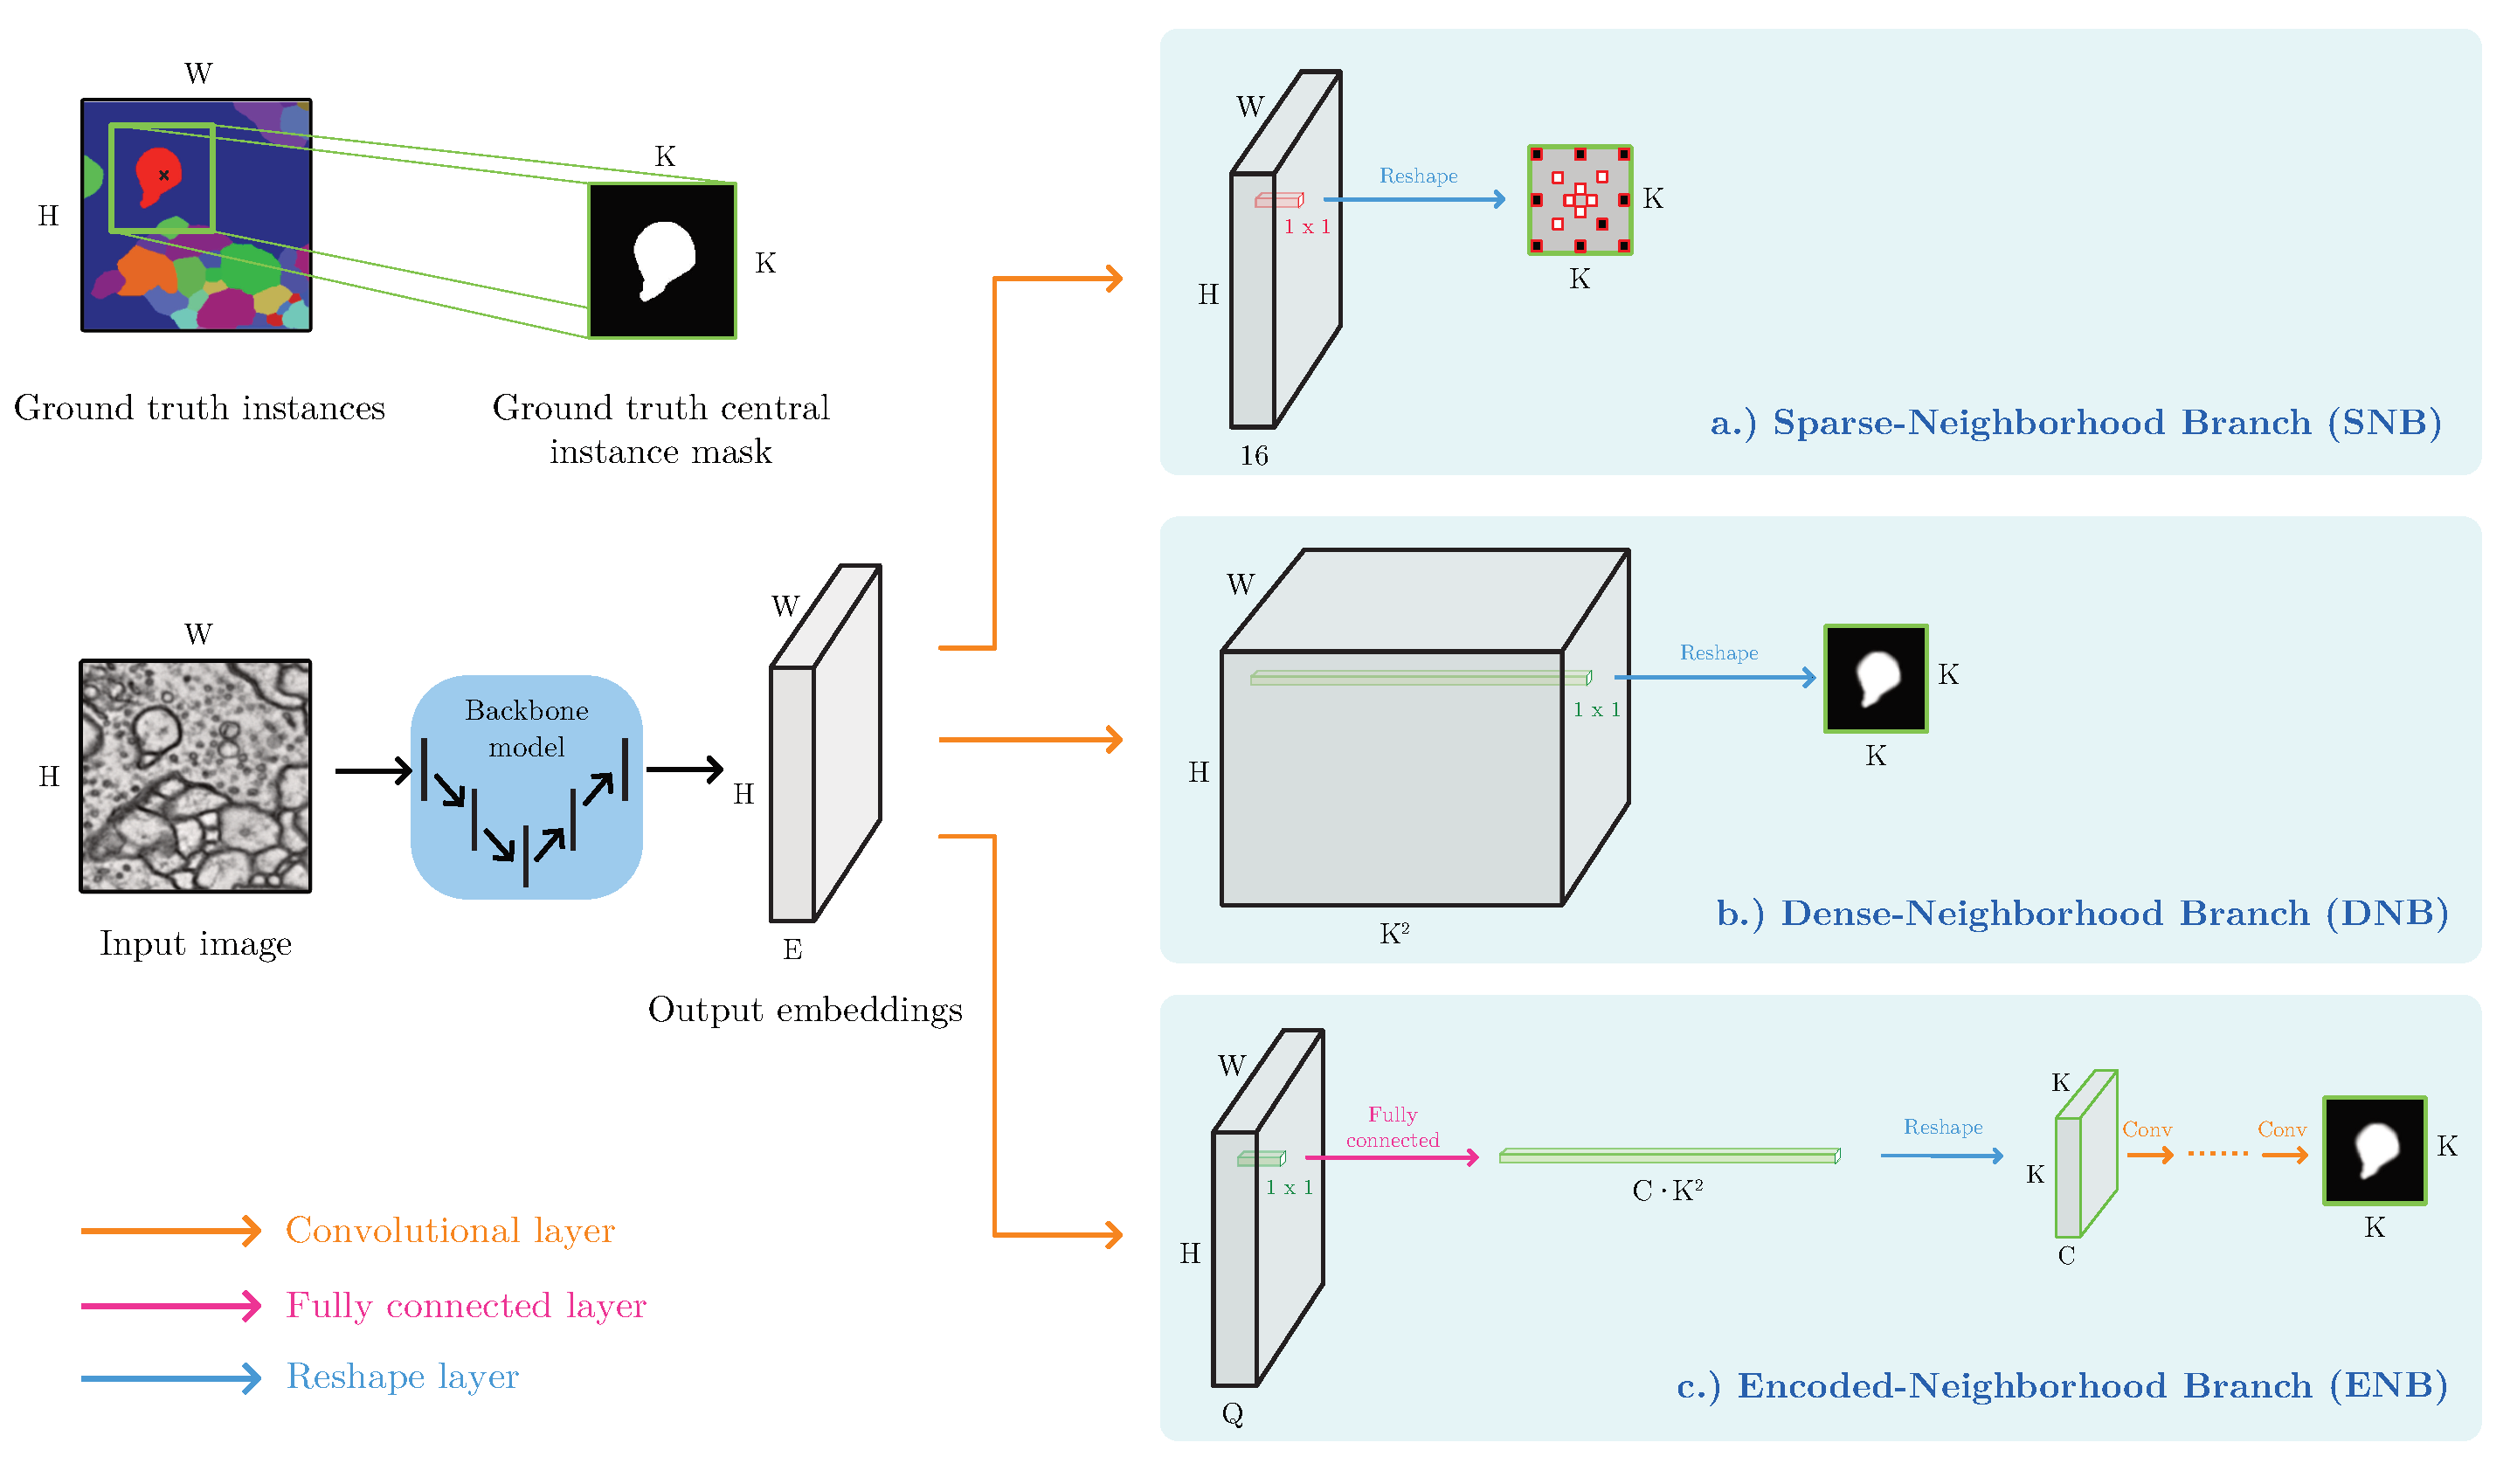
\includegraphics[width=\textwidth]{./figures/LSIMasks/main_fig.pdf} % 0.45
        \caption[Comparison between proposed and state-of-the-art methods]{Comparison between the proposed method and the strong baseline representing the current state-of-the-art. \textbf{Left}: At the top-left corner, an example of binary \maskname mask for a given ground truth label image; below, the backbone model predicts feature maps with the spatial dimensions of the input image. \textbf{Right}: a.) \emph{Sparse-neighborhood branch} used in the baseline model to predict affinities for a given sparse neighborhood structure; b) Simple generalization of the \emph{\sparseBr branch} to predict dense \maskname masks; c) Proposed \emph{\encBr branch} predicting \maskname masks in a low-dimensional latent space.}
    \label{fig:main_figure}
\end{figure}




\section{Introduction}\label{sec:intro}

\emph{Instance segmentation} is the computer vision task of assigning each pixel of an image to an instance, such as individual car, person or biological cell. %, where the number of instances is usually not known in advance. 
% The most success in instance segmentation (IS) has been achieved by applying deep learning. %\cite{he2017mask,romera2016recurrent,liu2018affinity}. 
There are two main types of successful deep learning approaches to instance segmentation: \emph{proposal-based} and \emph{proposal-free} methods. 
Recently, there has been a growing interest in the latter. Proposal-free methods do not require object detection and are preferred in imagery as studied here, in which object instances cannot be approximated by bounding boxes and are much larger than the field of view of the model.  

 
% A graph partitioning algorithm is used to obtain object instances.
Some recent successful proposal-free approaches \cite{januszewski2018high,liu2016multi,meirovitch2016multi} tackle instance segmentation by predicting, for a given patch of the input image, whether or not each pixel in the patch is part of the instance that covers the central pixel of the patch. 
This results a probability mask, which from now on we call \emph{\maskname mask}. These masks are then repeatedly predicted across the entire image, either in a sliding window style or by starting from a seed and then shifting the field of view depending on the previously predicted masks. 
Final object-instances are then obtained by aggregating predictions from overlapping masks which is in itself a nontrivial and interesting problem.
% In the following, we will refer to these patch predictions as \emph{\maskname masks}.

In this chapter, we introduce a new proposal-free segmentation method that is also based on predicting \maskname masks\footnote{For interesting, closely related but independent work, see \cite{hirsch2020patchperpix}.}.
% \footnote{Note to reviewers: As per ECCV reviewer instructions, there is no need to cite arxiv papers and they are not considered as prior \TODO{state of the art}. However, for maximum transparency and because we appreciate their fine work, we propose to keep footnote (1), hopefully upgraded to a full reference in our camera-ready version.}
However, our approach comes with four main advantages compared to previous methods.
Firstly, our model concurrently predicts all \maskname masks, one for each pixel, by using a fully-convolutional approach with much smaller computational footprint than previous methods, which iteratively predict one instance at the time, one mask after the other \cite{januszewski2018high,meirovitch2016multi}.
Secondly, our approach predicts \maskname masks in a low dimensional latent representation (see Fig. \ref{fig:main_figure}c), which results in great memory savings that are strictly required to apply the method to large volumetric images. 
Thirdly, the proposed approach aggregates predictions from overlapping \maskname masks without the need for any extra parameter or threshold and outputs predictions with associated uncertainty;
and, finally, all final object-instances are obtained concurrently, as opposed to previous methods predicting them one-by-one with subsequent conflict resolution. 
% by extracting a set of affinities that are then used as signed weights of a graph representing the image, so that each node corresponds to a pixel

% Despite the recent successful application of patch-based methods, so far no study has been conducted to compare them with 

Additionally, we systematically compare the proposed model with the current state-of-the-art proposal-free method both on natural and biological images \cite{liu2018affinity,Gao_2019_ICCV,lee2017superhuman,wolf2018mutex,bailoni2019generalized}. This strong baseline consists of a fully-convolutional network predicting, for each pixel, an arbitrary predefined set of short- and long-range affinities, i.e. neighborhood relations representing how likely it is for a pair of pixels to belong to the same object instance (see Fig. \ref{fig:main_figure}a). 

Our method achieves competitive scores on the challenging CREMI 2016 neuron segmentation benchmark. In our set of validation experiments, we show how predicting encoded \maskname masks always improves accuracy. Moreover, when predictions from overlapping masks are combined into edge weights of a graph that is subsequently partitioned, the result is a method that is strongly robust to noise and gives priority to predictions sharing the highest consensus across predicted masks. 
This parameter-free algorithm, for the first time, outperforms super-pixel based methods, which have so far been the default choice on the challenging data from the CREMI competition challenge.
 % and achieves competitive performances on the CREMI leader-board.


% In this work, we focus on a proposal-free method, where a Convolutional Neural Network (CNN) is trained to predict, for every pixel $i$ in the image, a patch of fixed size representing a probability mask of the instance object to which pixel $i$ belongs. The mask predicted in each patch is centered at the corresponding pixel $i$ and represents then a dense local neighborhood structure of pixel $i$. Whenever the object instance associated to pixel $i$ is bigger than the size of the patch, only a partial probability mask of the object is predicted. 
% In the following, we will call these masks as \patch or LSPM.

% [A naive way to predict one $K\times K$ \patch  for each pixel in an image would be to use a fully convolutional model with $K^2$ output channels, where each channel represents a pixel of the corresponding mask. However, this approach would not scale up well with increasing sizes $K$.]

% Our first contribution is a fully convolutional model that predicts, for every pixel $i$, a representation of the associated $i$-th self-probability mask in a lower dimensional space (see Fig. \ref{fig:main_figure}). This is possible due to the fact that, among all possible neighborhood structures represented by local self-probability masks, only few of them are associated to occurring ground truth binary masks. Thus, the information included in the predicted self-probability masks can be easily encoded in a lower dimensional latent space. 



% As a second contribution, we propose two methods for converting the predicted per-pixel self-probability masks into edge weights of a graph representing the image, so that each node corresponds to a pixel and a graph clustering algorithm is used to obtain the final instance segmentation... \TODO{Parameter-free alg. to compute edge weights; experiments; summary of sections}
% One of the two methods results in a pipeline that is as efficient as the currently winning method of the CREMI challenge \emph{(more efficient actually, because of LMC...), but achieves better accuracies and, as our results shows, outputs more consistent neighborhood structures...}.
% The second proposed method yields a parameter-free algorithm achieving competitive performances, yada yada yada... 


